\section{Introdução}

\subsection{Motivação e Contexto}

Úlceras em membros inferiores são lesões dermatológicas que tendem a se originar da deficiência no fluxo sanguíneo na região das feridas da pele~\cite{Pereira2011}.
Diversos fatores contribuem para sua formação, tais como diabetes, lesões, doenças vasculares, tumores, infecções e insuficiência venosa arterial~\cite{Ramelet2001}.
A Figura~\ref{fig:ulcerType} mostra os tipos mais comuns de úlceras. 
Para efeito desse trabalho serão considerados os tipos mais comuns de úlceras em membros inferiores, sendo elas as úlceras venosas, arteriais e neuropáticas, que representam cerca de 98\% dos casos de ulceração~\cite{Soutor2013}.

\begin{figure}[!htb]
    \centering
    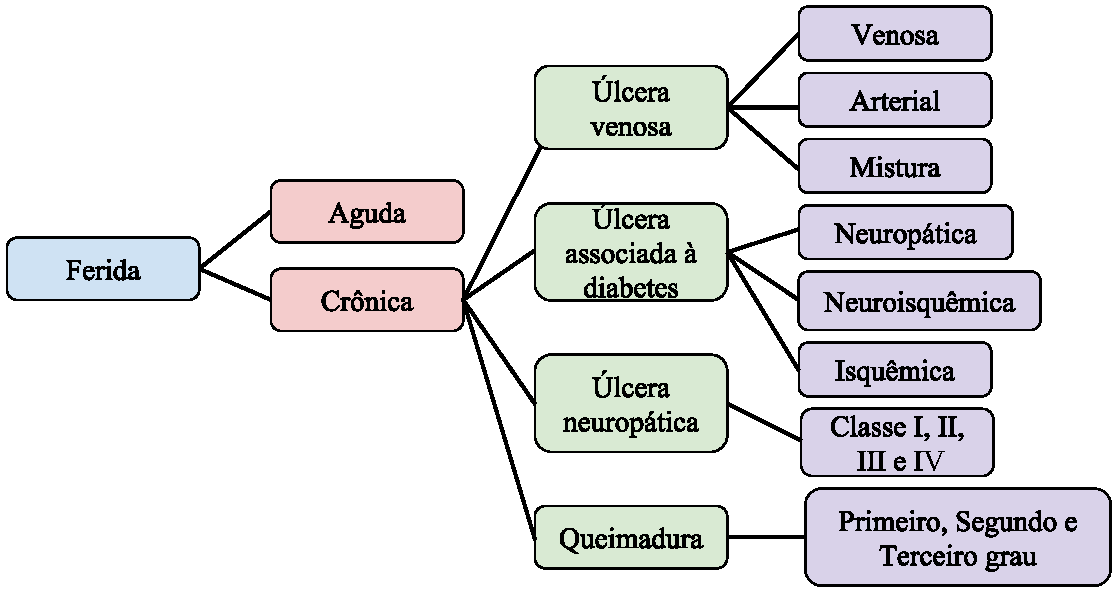
\includegraphics[scale=.7]{_fig/ulcerType.pdf}
    \caption[Classificação da tipos de lesões ulceradas.]{Classificação de tipos de lesões ulceradas.}
    \label{fig:ulcerType}
\end{figure}

Em particular, as úlceras que correspondem a ampla maioria dos casos de ulceração podem ser detalhadas de acordo com as seguintes características:

\begin{itemize}
\item \underline{Venosa (estase):} São lesões que surgem oriundas de veias varicosas e também de trombose venosa profunda. 
Podem evoluir para lesões crônicas, caso não se cicatrizem em poucas semanas~\cite{Abbade2005}.
Esse tipo resulta em uma morbidade significativa e ocasiona sequelas.

\item \underline{Arterial (isquêmica):} São lesões que têm sua origem associada a doenças arteriais periféricas, tabagismo e diabetes.
Geralmente o inicio da lesão é consequência da diminuição (ou obstrução total) do fluxo sanguíneo arterial nos membros inferiores.
Com o fluxo comprometido, há a necrose do tecido, o que causa a ulceração.
Esse tipo de úlcera costuma ser predominante em indivíduos do sexo masculino.

\item \underline{Neuropática:} São lesões que são comuns na região dos pés do paciente, área de pressão, como causas estão a diabete melito com dificuldade para cicatrização. 
Esse tipo de ulceração pode levar à amputação da região em vários casos.
\end{itemize}

O diagnóstico dessas lesões é realizado por dermatologistas, por meio dos chamados métodos macroscópico ou avaliações visuais da lesão, dado que o aspecto da úlcera expõe muitos de seus atributos importantes~\cite{Pereira2011}.
A precisão desse método de avaliação está associada à habilidade visual do especialista.
Entretanto, sabe-se que existem limitações associadas a esse método de avaliação, especialmente os ligados ao desgaste da rotina clínica e a variação da percepção de cada dermatologista~\cite{Maglogiannis2005}. 
Assim, o tratamento da ulceração pode ser afetado por essas imprecisões visuais, tornando necessário o uso de mecanismo intrusivos de avaliação, como a biópsia.

O tratamento para a lesão visa fechar e evitar o reaparecimento da úlcera.
Existem diversos procedimentos para a cicatrização da lesão, como, por exemplo: intervenção cirúrgica, medicamentos e terapias. 
Esses métodos, são normalmente combinados de acordo com o prognóstico visual do especialista.
Após o tratamento da lesão, a preocupação passa ser com o seu reaparecimento, com maior probabilidade de ocorrência nos primeiros anos (pós-tratamento).
Portanto devem-se tomar medidas de prevenção, tais como, fisioterapia e o uso de meias elásticas de compressão médica.
Um fato importante é que os procedimentos preventivos também variam de acordo com o tipo da úlcera dermatológica~\cite{Abbade2005}.

Visualmente, o aspecto da úlcera é caraterizado por seu formato irregular, com bordas nítidas e rígidas. 
Em estados iniciais, a ulceração, apresenta-se como uma lesão superficial, que tende a se aprofundar com o decorrer do tempo.
A fisionomia da úlcera também demonstra particularidades, como sua composição, textura e tonalidade \cite{Dorileo2010}. 
Nesta fisionomia, é possível definir quais as particularidades da lesão e os tecidos que a compõem, \textit{i.e.}, granulação, fibrina, necrose e tecido misto~\cite{Pereyra2014}. 
O aspecto de cada tecido e suas particularidades estão ilustrados na Figura \ref{figTecidos}, na qual os tecidos indicam os estágios de cicatrização da lesão. 
Esses tipos de tecido podem ser descritos como: 

\begin{itemize}
\item \underline{Granulação:} Inclui a composição de brotos capilares, que se organizam de diversas formas, e se caracteriza por estar presente durante o início da cicatrização da lesão; 

\item \underline{Fibrina:} É uma agregação das plaquetas e de líquidos serosos na região onde houve rompimento de vasos sanguíneos.
Esse tecido constitui um tipo de coágulo sanguíneo; 

\item \underline{Necrose:} É um tecido composto por células mortas e descartadas, que pode indicar como a úlcera está atingindo os tecidos orgânicos;

\item \underline{Tecido misto:} São compostos de uma mistura dos três tecidos anteriores, que ocorrem ao mesmo tempo.
\end{itemize}


Cada tecido possui seus atributos característicos em termos de cor e textura predominante \cite{Pereira2011}.
Por exemplo, tecidos granulosos são compostos pela cor vermelha; tecidos de fibrina predominantemente formados pela tonalidade amarelada; tecidos necrose tem sua formação caraterizada pela cor preta e marrom escuro. Por último, a mistura de tecidos é composta diversos fragmentos de cores e texturas \cite{Chino2018}.   

Portanto, com o objetivo de auxiliar a análise macroscópica do dermatologista feita para a lesão de úlcera, nossa proposta é a definição de um sistema de processamento de imagens digitais automatizado~\cite{Gonzalez2008}.
Uma consequência indireta, porém benéfica, é que o uso desses sistemas permitem tanto reproduzir a análise, quando justificar em termos algorítmicos o método de detecção.
Abordagens existentes identificam cores e texturas predominantes na lesão e as associam com o tipo de tecido \cite{Chino2018,Blanco2016}.
O método a ser discutido neste trabalho é complementar ao uso dessas abordagens, no sentido que não assume a existência de nenhuma classe de tecido, mas os agrupa de acordo com padrões implícitos nos tecidos lesionados.


\subsection{Modelo de quatro cores}

\begin{figure}[!t]
    \centering
    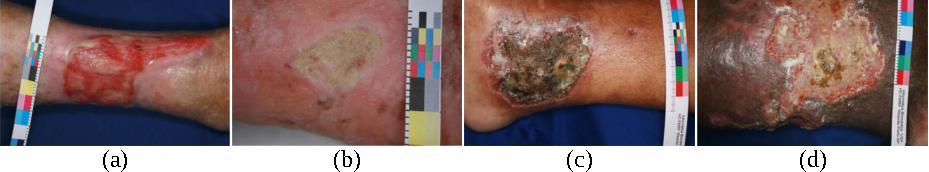
\includegraphics[scale=1]{_fig/tecidos.pdf}
    \caption[Exemplos de úlceras]{Exemplos de úlceras. 
    (a)~Tecidos de granulação. 
    (b)~Tecidos de fibrina. 
    (c)~Tecidos necrosados.
    (d)~Tecidos mistos. 
    Adaptado de \citeonline{Pereira2011} }
    \label{figTecidos}
\end{figure}

Métodos de processamento de imagens aplicados no domínio de úlceras dermatológicas, visam rotular os diferentes tipos de tecidos da lesão, de acordo com sua cor e  textura.
Levando em conta que os tecidos qualificados na análise macroscópica incluem \textit{granulação, fibrina, necrose} e \textit{misto}, é possível determinar diversas etapas com o objetivo auxiliar o diagnóstico e tratamento de úlceras em membros inferiores~\cite{Blanco2016}. 
O processo do tratamento é divido em três etapas, de acordo com a quantidade de cada um dos tecidos:

\begin{enumerate}

\item \underline{Inflamação:} É a primeira resposta protetora do sistema imunológico, resultando em uma vermelhidão causada pelo aumento do fluxo sanguíneo e demais fluxos corporais que migram para região da ferida e podem aumentar a temperatura da região. 

\item \underline{Formação de tecido:} Caracterizada por brotos capilares e fibroblastos. 
Trata da formação de tecido de granulação, que dá inicio ao processo de cicatrização (que não é, necessariamente, definitivo). 

\item \underline{Remodelagem}: Essa estágio indica a remodelagem da cicatrização e a re-e\-pi\-te\-li\-za\-ção, que é o crescimento de tecido orgânico (pele saudável) nas bordas da feridas, sendo um acontecimento final no processo de reparo.

\end{enumerate}

\subsection{Diagnóstico Assistido por Computador}

Sistemas de Diagnóstico Assistido por Computador (CAD - \textit{Computer-Aided Diagnosis}) traz em diversas vantagens à avaliação macroscópica, minimizando eventuais desvantagens à percepção do especialista no momento da avaliação visual, tais como: iluminação do ambiente, desgaste físico e diagnósticos prévio divergente entre diferentes profissionais~\cite{Maglogiannis2005}. 
O propósito de um sistema CAD nesse caso, é auxiliar no diagnóstico e o prognóstico de lesões.
Sistemas CAD baseados puramente em aprendizado de máquina já são capazes de identificar e diagnosticar lesões com qualidade próxima ou superior a dermatologistas humanos~\cite{Esteva2017}.
Entretanto, para úlceras dermatológicas, objeto de estudo desse trabalho, ainda não existem sistemas CAD com resultados dessa magnitude, e proporcionar maior agilidade, eficiência, confiabilidade replicação fácil dos prognósticos indicados ainda é uma dificuldade~\cite{Blanco2016,Kavitha2017,Chino2018}.
Uma ferramenta CAD aplicada ao domínio de úlceras dermatológicas deve ser focada na segmentação dos tecidos para auxiliar o especialista humano no diagnóstico da lesão~\cite{Oduncu2004,Pereyra2014}. 
De acordo com \citeonline{Bedo2015a} os pontos e objetivos da maioria das ferramentas CAD para úlceras dermatológicas na literatura se baseiam em quatro processos:

\begin{itemize}
    
    \item \underline{Segmentação de imagem:} Processo de separação da área de interesse (pele) e descarte de partes irrelevantes (fundo), bem como separação de possíveis tipos de tecidos lesionados;
    
    \item \underline{Extração de características:} Processo usado para representar segmentos de uma imagem, como vetores numéricos multidimensionais;
    
    \item \underline{Seleção de características:} Processo usado para selecionar as dimensões mais representativas dos vetores numéricos multidimensionais que foram extraídos (dos pedaços) da imagem ou fotografia original da úlcera; 
    
    \item \underline{Classificação da imagem:} É o processo utilizado para rotular cada um dos pedaços da imagem representados como vetores de dimensões significativas.
\end{itemize}

Ainda que esses quatro processos sejam o centro do funcionamento de sistemas CAD, técnicas de processamento de imagens podem ser empregadas com a finalidade de melhorar o resultado em qualquer estágio do processamento e auxiliar na identificação de particularidades das lesões~\cite{Gonzalez2008}. 
Portanto, um sistema CAD para úlceras dermatológicas deve ter por objetivo fornecer uma solução para processamento e análise de imagens médicas específicas.
Uma limitação no processamento é a aquisição da imagem, que no caso de úlceras dermatológicas, pode ser contornado com o uso de um plano de fundo, ângulo, foco e distância fixos~\cite{Pereyra2014}.  

Assim, a solução proposta deve permitir a separação e quantificação de conteúdos relevantes das imagens, como as regiões da úlcera. 
Para cada região dever ser possível determinar padrões dos tecidos presentes na lesão. 
A abordagem CAD proposta será inspiradas em sistemas de trabalhos anteriores~\cite{Pereira2011,Blanco2016,Kavitha2017,Chino2018}.
Estes sistemas já auxiliam o dermatologista ao informar medidas estatísticas e ao recuperar casos similares por conteúdo. 

No entanto, nenhum dos estudos anteriores analisou o problema de segmentação de úlceras dermatológicas tanto da perspectiva supervisionada quanto da perspectiva não-supervisionada, no sentido de usar uma abordagem em duas fases para separar conteúdos relevantes da lesão e detecção de padrões em trechos de tecidos \textit{não lesionados}.
Em particular, os trabalhos existentes, não combinam técnicas de pré-processamento e classificadores supervisionados para descartar partes irrelevantes da área da lesão, mas sim para rotular as áreas lesionadas em si~\cite{Chino2018}.
Nossa premissa é, primeiro, combinar esses métodos para descartar padrões desimportantes para a análise dos tecidos ulcerados e, só depois, buscar padrões nos tecidos segmentados sem considerar rótulos ou comportamentos específicos.


\subsection{Objetivos}

Há duas metas essenciais para que se possa atingir o objetivo proposto. 
A primeira é a separação entre pele do paciente e o fundo da imagem, enquanto que a segunda é a de agrupar os tecidos de acordo com padrões implícitos entre eles.
Portanto, os objetivos específicos desse trabalho, consistem em:

\begin{enumerate}

\item Segmentação da imagem entre pele e outros -- Essa tarefa é abordada considerando técnicas de processamento de imagens e de aprendizado de máquina supervisionado. 

\item Agrupamento dos tecidos lesionados -- Após a eliminação de áreas desimportantes da análise, buscar-se-á combinar técnicas de processamento de imagens (geração de \textit{superpixels}) e técnicas de aprendizagem de máquina não-supervisionadas para agrupar os tecidos com padrões similares, porém não explícitos.

\end{enumerate}

\subsection{Organização da Monografia}
Esse documento está organizado em cinco capítulos.
Além desse, os demais capítulos incluem o seguinte conteúdo:
\begin{itemize}
    \item O Capítulo~\ref{sec:background} apresenta o arcabouço conceitual sobre os métodos empregados e uma comparação dos trabalhos relacionados.
    São revisados conceitos de morfologia matemática, classificação e agrupamento, com destaque especial para o método de agrupamento particional DBSCAN.
    \item O Capítulo~\ref{sec:methods} explica a metodologia adotada, as imagens utilizadas, a abordagem implementada, além dos testes realizados e resultados obtidos.
    São discutidas duas soluções implementadas, uma solução \textit{ad-hoc} baseada em processamento de imagens e uma alternativa baseada em aprendizado de máquina.
    \item O Capítulo~\ref{sec:exp_result} apresenta os resultados sobre avaliações experimentais sobre os métodos propostos.
    As avaliações são conduzidas sobre um conjunto de dados real.
    \item O Capítulo~\ref{sec:conclusion} apresenta as conclusões derivadas das observações realizadas, um resumo das publicações derivadas e direções sobre trabalhos futuros.
\end{itemize}

